\documentclass[10pt]{article}
\usepackage{amsmath}
\usepackage{geometry}
\usepackage{fancybox}
\usepackage{amsfonts}
\usepackage{amsbsy}
\usepackage{tikz}
\usepackage{listings}
\usepackage{amsthm}
\geometry{
a4paper,
total={170mm,257mm},
left=20mm,
top=10mm,
bottom=15mm
}
\usepackage{color}
\definecolor{codegreen}{rgb}{0,0.6,0}
\definecolor{codegray}{rgb}{0.5,0.5,0.5}
\definecolor{codepurple}{rgb}{0.58,0,0.82}
\definecolor{backcolour}{rgb}{0.95,0.95,0.92}

\linespread{1.3}

\title{CSC263H1 Assignment 6}
\author{Jiatao Xiang, Xu Wang, Huakun Shen}
\date{March 28th, 2019}

\begin{document}

\lstdefinestyle{mystyle}{
    backgroundcolor=\color{backcolour},   
    commentstyle=\color{codegreen},
    keywordstyle=\color{magenta},
    numberstyle=\tiny\color{codegray},
    stringstyle=\color{codepurple},
    basicstyle=\footnotesize,
    breakatwhitespace=false,         
    breaklines=true,                 
    captionpos=b,                    
    keepspaces=true,                 
    numbers=left,                    
    numbersep=5pt,                  
    showspaces=false,                
    showstringspaces=false,
    showtabs=false,                  
    tabsize=4
}
\lstset{style=mystyle}
\maketitle
\section*{Question 1}
\begin{itemize}
\item[a.]
\end{itemize}
\ovalbox{
\begin{tikzpicture}[level/.style={sibling distance=60mm/#1}]
\node [circle,draw, label=right:$1/12$] (z){$1$}
  child {node [circle,draw, label=right:$2/3$] (lz) {$6$}}
  child {node [circle,draw, label=right:$4/11$] (rz) {$4$}
    child {node [circle,draw, label=right:$5/8$] (rlz) {$5$}
    	child {node [circle, draw, label=right:$6/7$] (rllz) {$2$}}
		child[fill=none]{edge from parent[draw=none]}     
    }
  child {node [circle,draw, label=right:$9/10$] (rrz) {$7$}
	}
};
\end{tikzpicture}
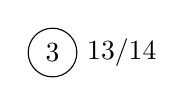
\begin{tikzpicture}[level/.style={sibling distance=60mm/#1}]
\node [circle,draw, label=right:$13/14$] (z){$3$};
\end{tikzpicture}
}
\begin{itemize}
\item[b.] Forward edge: 7, Back edge: 0, Cross edge: 5.
\item[c.] Use white-path theorem and parenthesis theorem.\\
To prove that it is possible to take all the courses
in a sequential order that satisfies all the prerequisite requirements, we have to prove that there are not two courses that are prerequisites of each other. \\
Suppose $u$ and $v$ are two nodes in $G$ that represent 2 courses, then $u$ is a prerequisite of $v$ if and only if $u.f>v.f$. So it is suffice to show that for every edge $(u,v)\in E$, $u.f>v.f$.
\begin{proof} To prove that $\forall$ edge $(u,v)\in E$, $u.f>v.f$.\\
\textbf{Case 1:} $(u, v)$ is a back edge\\
We know that, in the DFS forest above, there is no back edge, i.e. there is not cycle, so that there is not 2 courses being the prerequisites of each other.\\
\textbf{Case 2:} $(u,v)$ is a forward edge or tree edge\\
Then $v$ is a descendant of $u$. By parenthesis theorem, $u.d<v.d<v.f<u.f\Rightarrow u.f>v.f$\\
\textbf{Case 3:} $(u,v)$ is a cross edge\\
Then $u$ and $v$ are not descendants of one another, i.e. there is no prerequisite-relationship between $u$ and $v$, which means the order doesn't matter for these two courses. So we can make $u.f>v.f$ (i.e. take $u$ before $v$).\\
\end{proof}
\item[d.] $3\rightarrow 1\rightarrow 4\rightarrow 7\rightarrow 5\rightarrow 2\rightarrow 6$, in this ordering, each vertex's finish time is greater than the finish time of its next node.
\item[e.]
\end{itemize}

\section*{Question 2}


\section*{Question 3}


\end{document}
